\section{Orthogonalprojektion im $\mathbb{R}^n$ (+)}\label{MA2-orthogonalprojektion}

\begin{table}[H]
  \centering
  \begin{tabularx}{\textwidth}{@{}>{\raggedright\arraybackslash}X r@{}}
    \toprule
    \multicolumn{2}{c}{\textbf{�bersicht �ber Lernziele und Voraussetzungen}}\\
    \midrule
    \textbf{Lernziele} & \\[.5\normalbaselineskip]
    \tabitem das Prinzip �Minimalabstand $\Leftrightarrow$ Orthogonalit�t� geometrisch erkl�ren & \\
    \tabitem die Orthogonalprojektion eines Vektors auf einen Unterraum interpretieren & \\
    \tabitem ein �berbestimmtes lineares Gleichungssystem als Approximationsproblem formulieren & \\
    \tabitem die Normalengleichung $A^\top A\,\vec x = A^\top \vec b$ herleiten und anwenden & \\
    \tabitem das Residuum als orthogonalen Fehlervektor im Bildraum von $A$ deuten & \\[.5\normalbaselineskip]
    \midrule
    \textbf{Voraussetzungen} & \\[.5\normalbaselineskip]
    \tabitem Rang und Bildraum einer Matrix bestimmen k�nnen & \abschnittsverweis{MA1-lineare-gleichungssysteme}  \\
    \tabitem mit Skalarprodukten und Normen im $\mathbb R^n$ umgehen k�nnen &  \abschnittsverweis{MA1-vektoren} \\
    \tabitem Matrizen transponieren und Matrix-Vektor-Produkte berechnen k�nnen & \abschnittsverweis{MA1-matrizen}\\
    \bottomrule
  \end{tabularx}
\end{table}

\noindent \ifintegriereaufgaben Die �bungsaufgaben zum Thema finden Sie \hyperref[MA2-orthogonalprojektion-aufgaben]{hier}.
\vspace{0.3cm}
\hrule
\fi


Die bei der Fourier-Approximation beobachtete Struktur ist kein Spezialph�nomen des Funktionenraums.

Sie tritt immer dann auf, wenn ein Element eines Vektorraums durch Elemente eines Unterraums m�glichst gut approximiert werden soll.

Die zugrunde liegende Idee lautet:

\[
\text{Abstand minimiert}
\quad \Longleftrightarrow \quad
\text{Orthogonalit�tsrelation erf�llt} \,.
\]


Diese Struktur gilt in jedem Raum mit Skalarprodukt - insbesondere also auch im endlichdimensionalen Raum $\mathbb{R}^n$.

Gegeben sei ein Unterraum $V \subset \mathbb{R}^n$ und ein Vektor $\vec b \in \mathbb{R}^n$. Gesucht ist derjenige Vektor $\vec v \in V$ mit

\[
	\|\vec b - \vec v\| = \min_{\vec u \in V} \|\vec b - \vec u\|\,.
\]

Wie im Funktionenraum gilt:

\[
	\vec b - \vec v \perp V\,.
\]

\begin{exabox}{Geometrische Interpretation}{}
\begin{minipage}{0.3\textwidth}
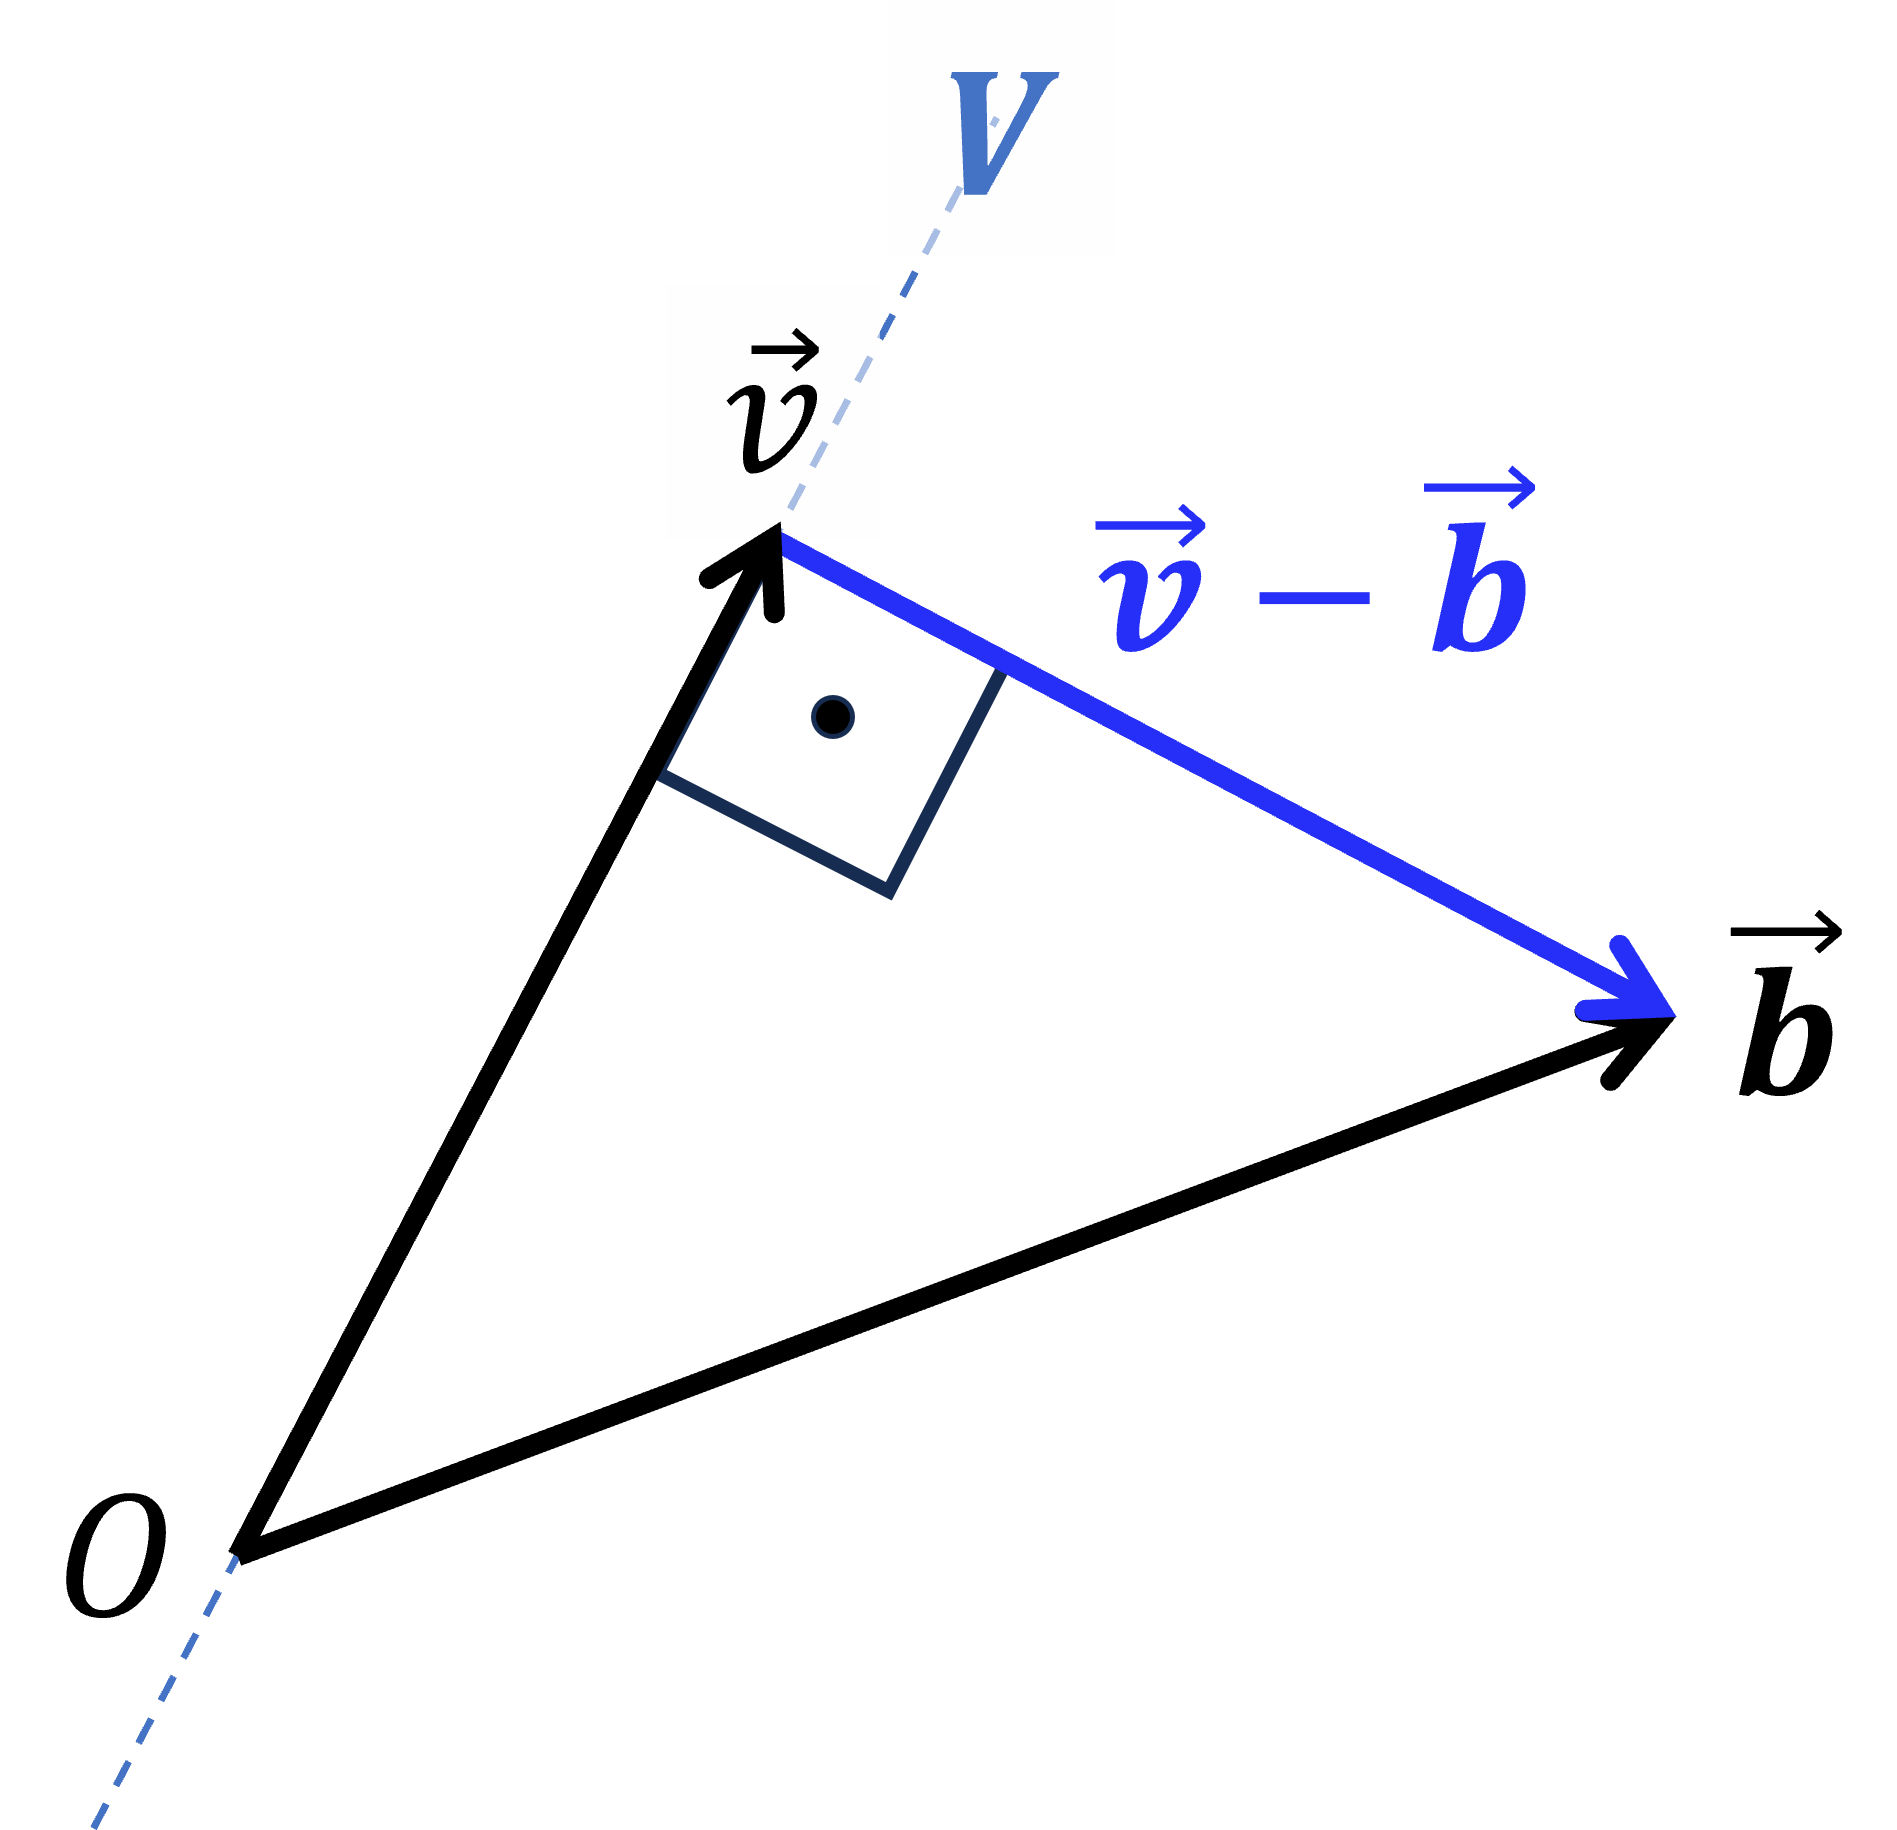
\includegraphics[width=\textwidth]{../Mathematik_2/Bilder/orthogonalprojektion_geometrie_des_residuums.png}
\end{minipage}
\begin{minipage}{0.7\textwidth}
	\begin{itemize}
		\item Das Residuum (der Fehler- oder Abstandsvektor)  \(\vec b - \vec v\) steht senkrecht auf dem gesamten Unterraum.
		\item Die Orthogonalit�t des Residuums charakterisiert den Punkt minimalen Abstands:
	\end{itemize}
\end{minipage}
\end{exabox}

\subsection*{Anwendung: L�sung eines �berbestimmten Gleichungssystems}

Betrachten wir nun ein lineares Gleichungssystem

\[
	A \vec x = \vec b, \qquad A \in \mathbb{R}^{n \times m}, \; n>m \,.
\]

Ist das System nicht l�sbar, so liegt $\vec b$ nicht im Bildraum von $A$:

\[
	\vec b \notin \mathrm{im}(A)\,.
\]

Starten wir mit einer konkreten, sehr einfachen Aufgabe: gesucht sind Zahlen \(x_1, \,  x_2 \in \mathbb R\), die folgende Gleichungen simultan erf�llen \begin{equation}\label{Beispiel1} \begin{cases} \begin{array}{rcr c l } x_1 &&&=& 1\,, \\& & x_2 &=& 1\,, \\ x_1 &+&x_2 &=& 1\end{array} \end{cases} \Rightarrow  \quad \begin{array}{cccc}
	\left( \begin{array}{cc}
			1 & 0   \\
			0 & 1   \\
			1 & 1
\end{array}\right)& \left( \begin{array}{c}x_1 \\x_2\end{array} \right) &=&  \left( \begin{array}{c} 1 \\ 1 \\ 1 \end{array}\right) \\ \underbrace{\quad\quad\quad\quad\quad\quad}_{\displaystyle{=A}} &\underbrace{\quad\quad\quad}_{\displaystyle{=\vec x}} &&  \underbrace{\quad\quad\quad}_{\displaystyle{=\vec b}} \end{array}
\end{equation}
Um den Gau�-Algorithmus anzuwenden betrachten wir die erweitertete Koeffizientenmatrix \( A_{\vec b} = \left( A|\vec b\right)\) und bringen die Matrix zun�chst auf Trapezform:

\vspace{0.1cm}
\begin{exabox}{L�sungsversuch �berbestimmtes Gleichungssystem}{ }
	\[ \begin{array}{r c l} \textnormal{Ausgangsgleichung} & & \left( \begin{array}{cc|c}
			1 & 0   & 1 \\
			0 & 1   & 1\\
	1 & 1 & 1 \end{array}\right)\\
	\textnormal{Trapezform} & \Leftrightarrow &
\left( \begin{array}{cc|c}
		1 & 0 & 1\\
		0 & 1 & 1 \\
		0 & 0 & 1
\end{array} \right) \Rightarrow \textnormal{Aufl�sen klappt nicht!} \end{array}\]
\vspace{0.1cm}
\begin{itemize}
	\item[\(\Rightarrow\)] Die L�sbarkeitsbedingung ist nicht erf�llt: \(\mathrm{rang}(A) \not=\mathrm{rang}(A_{\vec b})\).
	\item[\(\Rightarrow\)] Das Gleichungssystem ist nicht l�sbar, die L�sungsmenge ist leer!
\end{itemize}
\end{exabox}
\bigskip


Die Vektoren $A\vec x$ bilden einen Unterraum des $\mathbb{R}^n$, den Bildraum \(\mathrm{im}(A)\). Was k�nnen wir tun? Wir suchen daher denjenigen Vektor $A\vec x_*$, der $\vec b$ am n�chsten kommt.

\begin{exabox}{Nichtl�sbares Gleichungssystem}{}
\begin{minipage}{0.3\textwidth}
	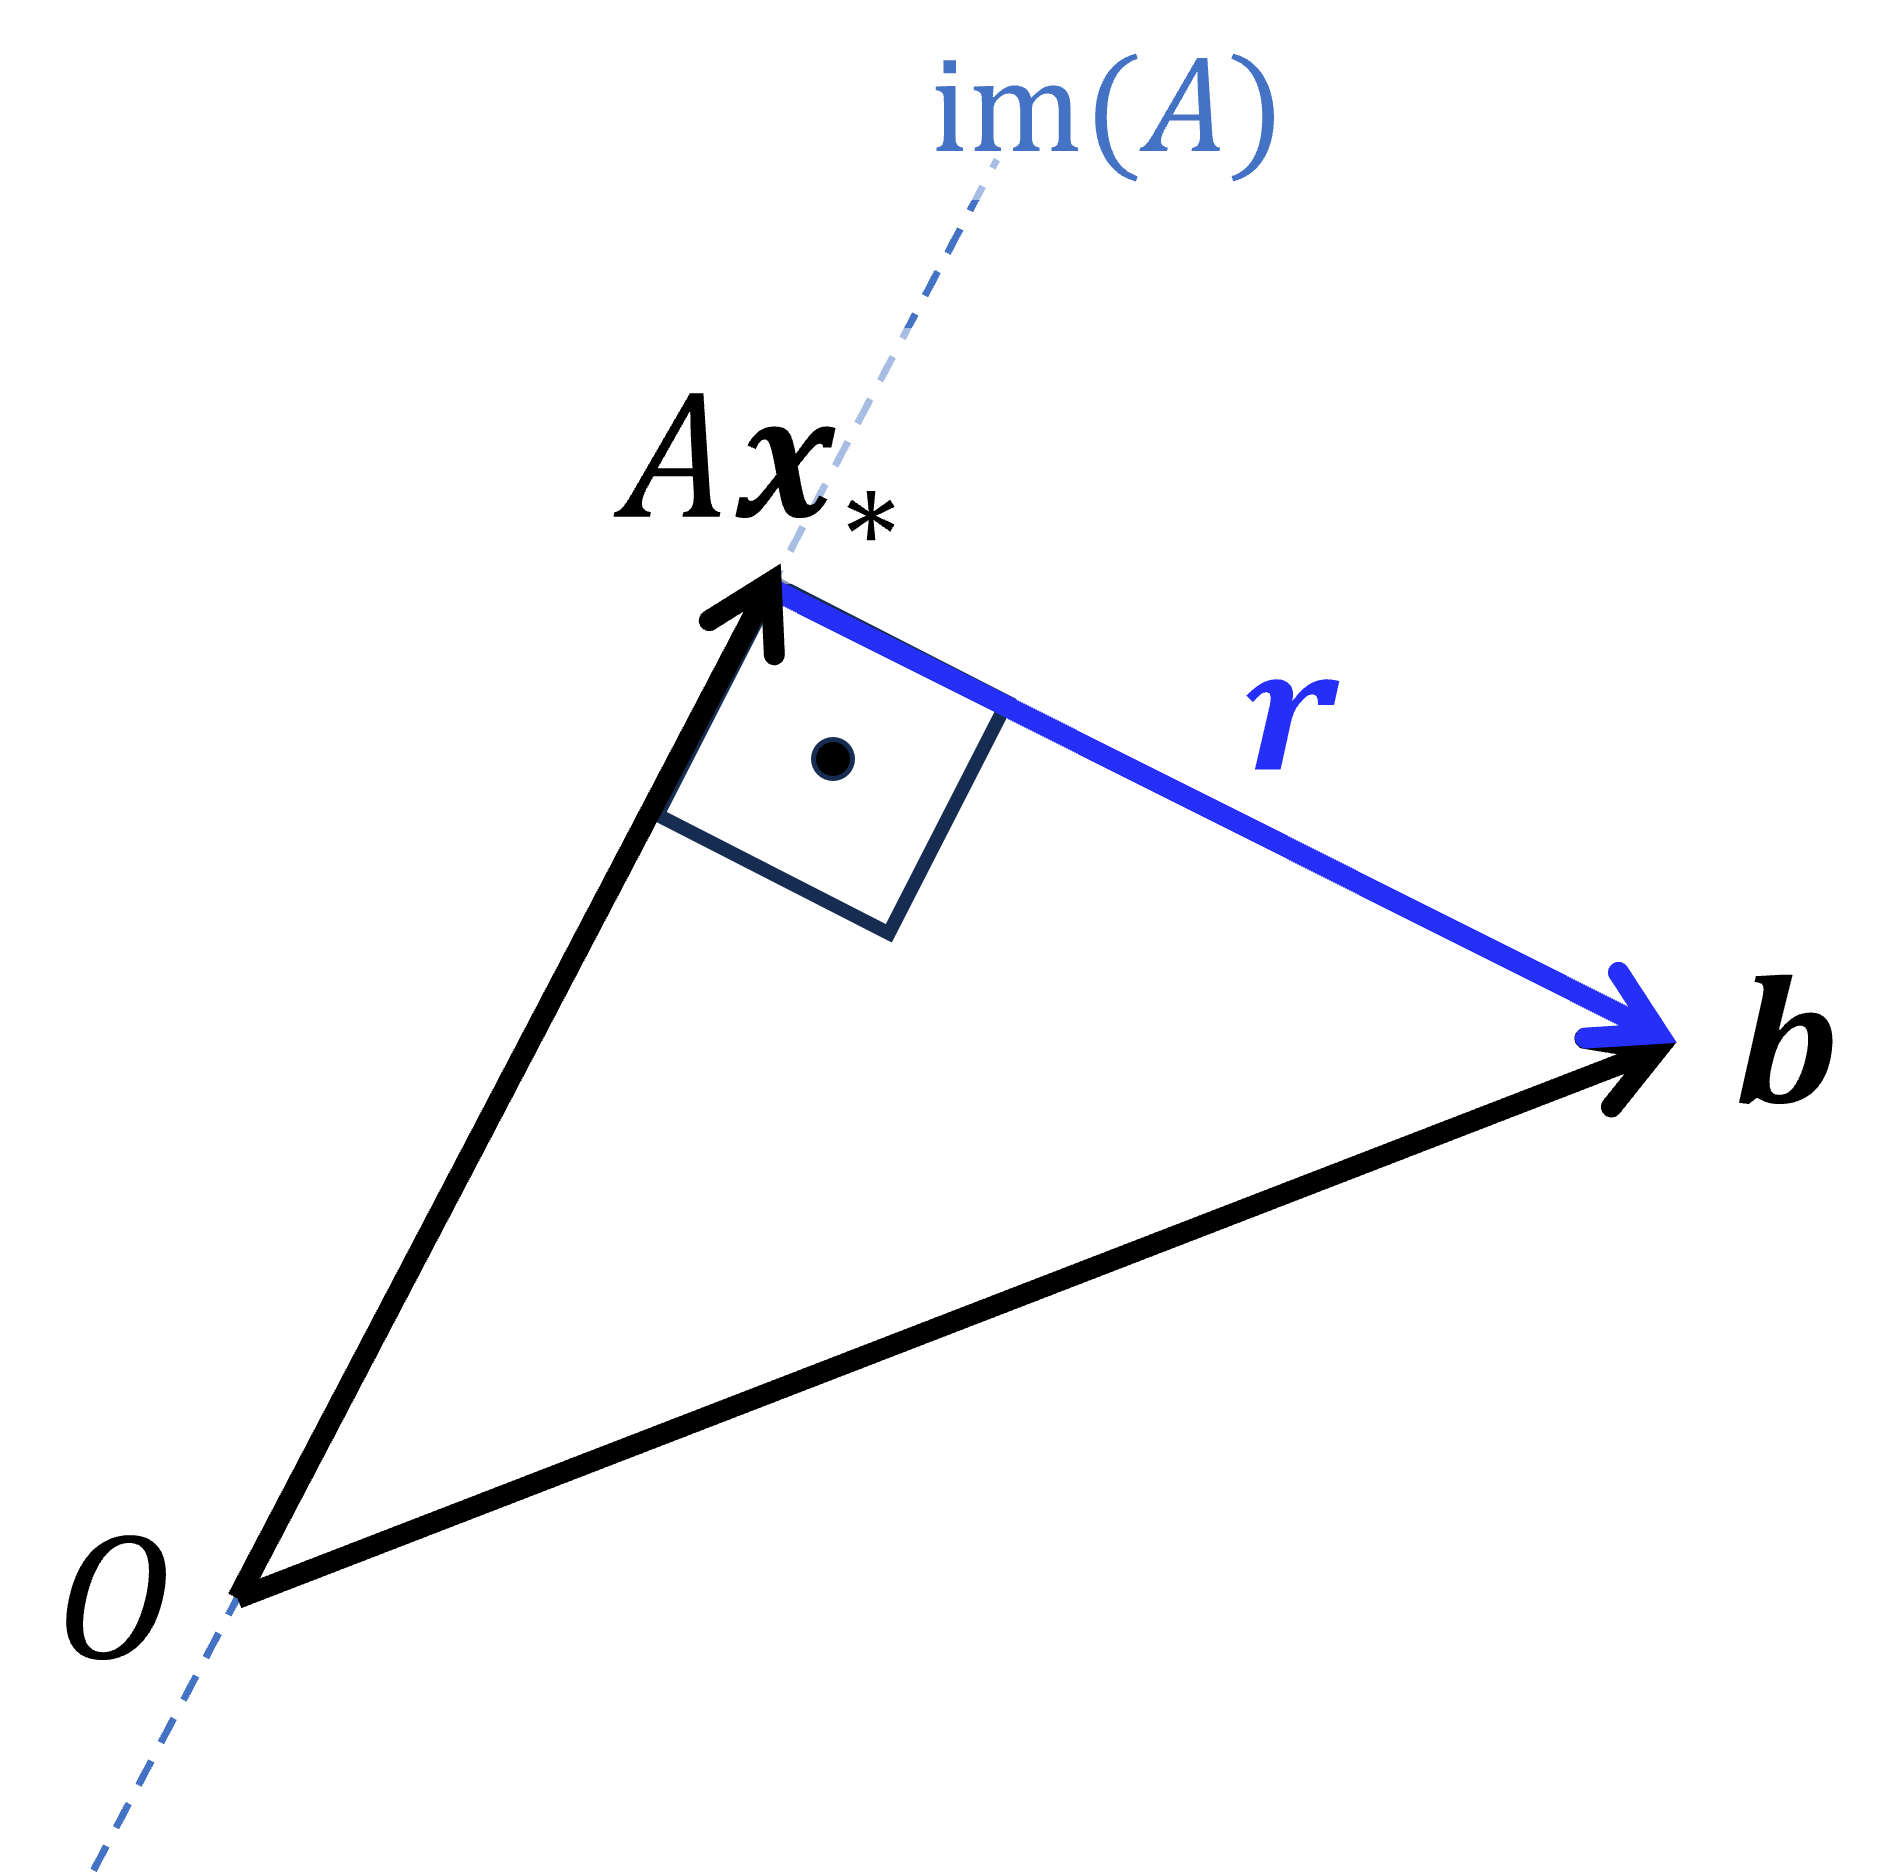
\includegraphics[width=\textwidth]{../Mathematik_2/Bilder/ausgleichsrechnung_residuum_orthogonal_zum_bildraum.png}
%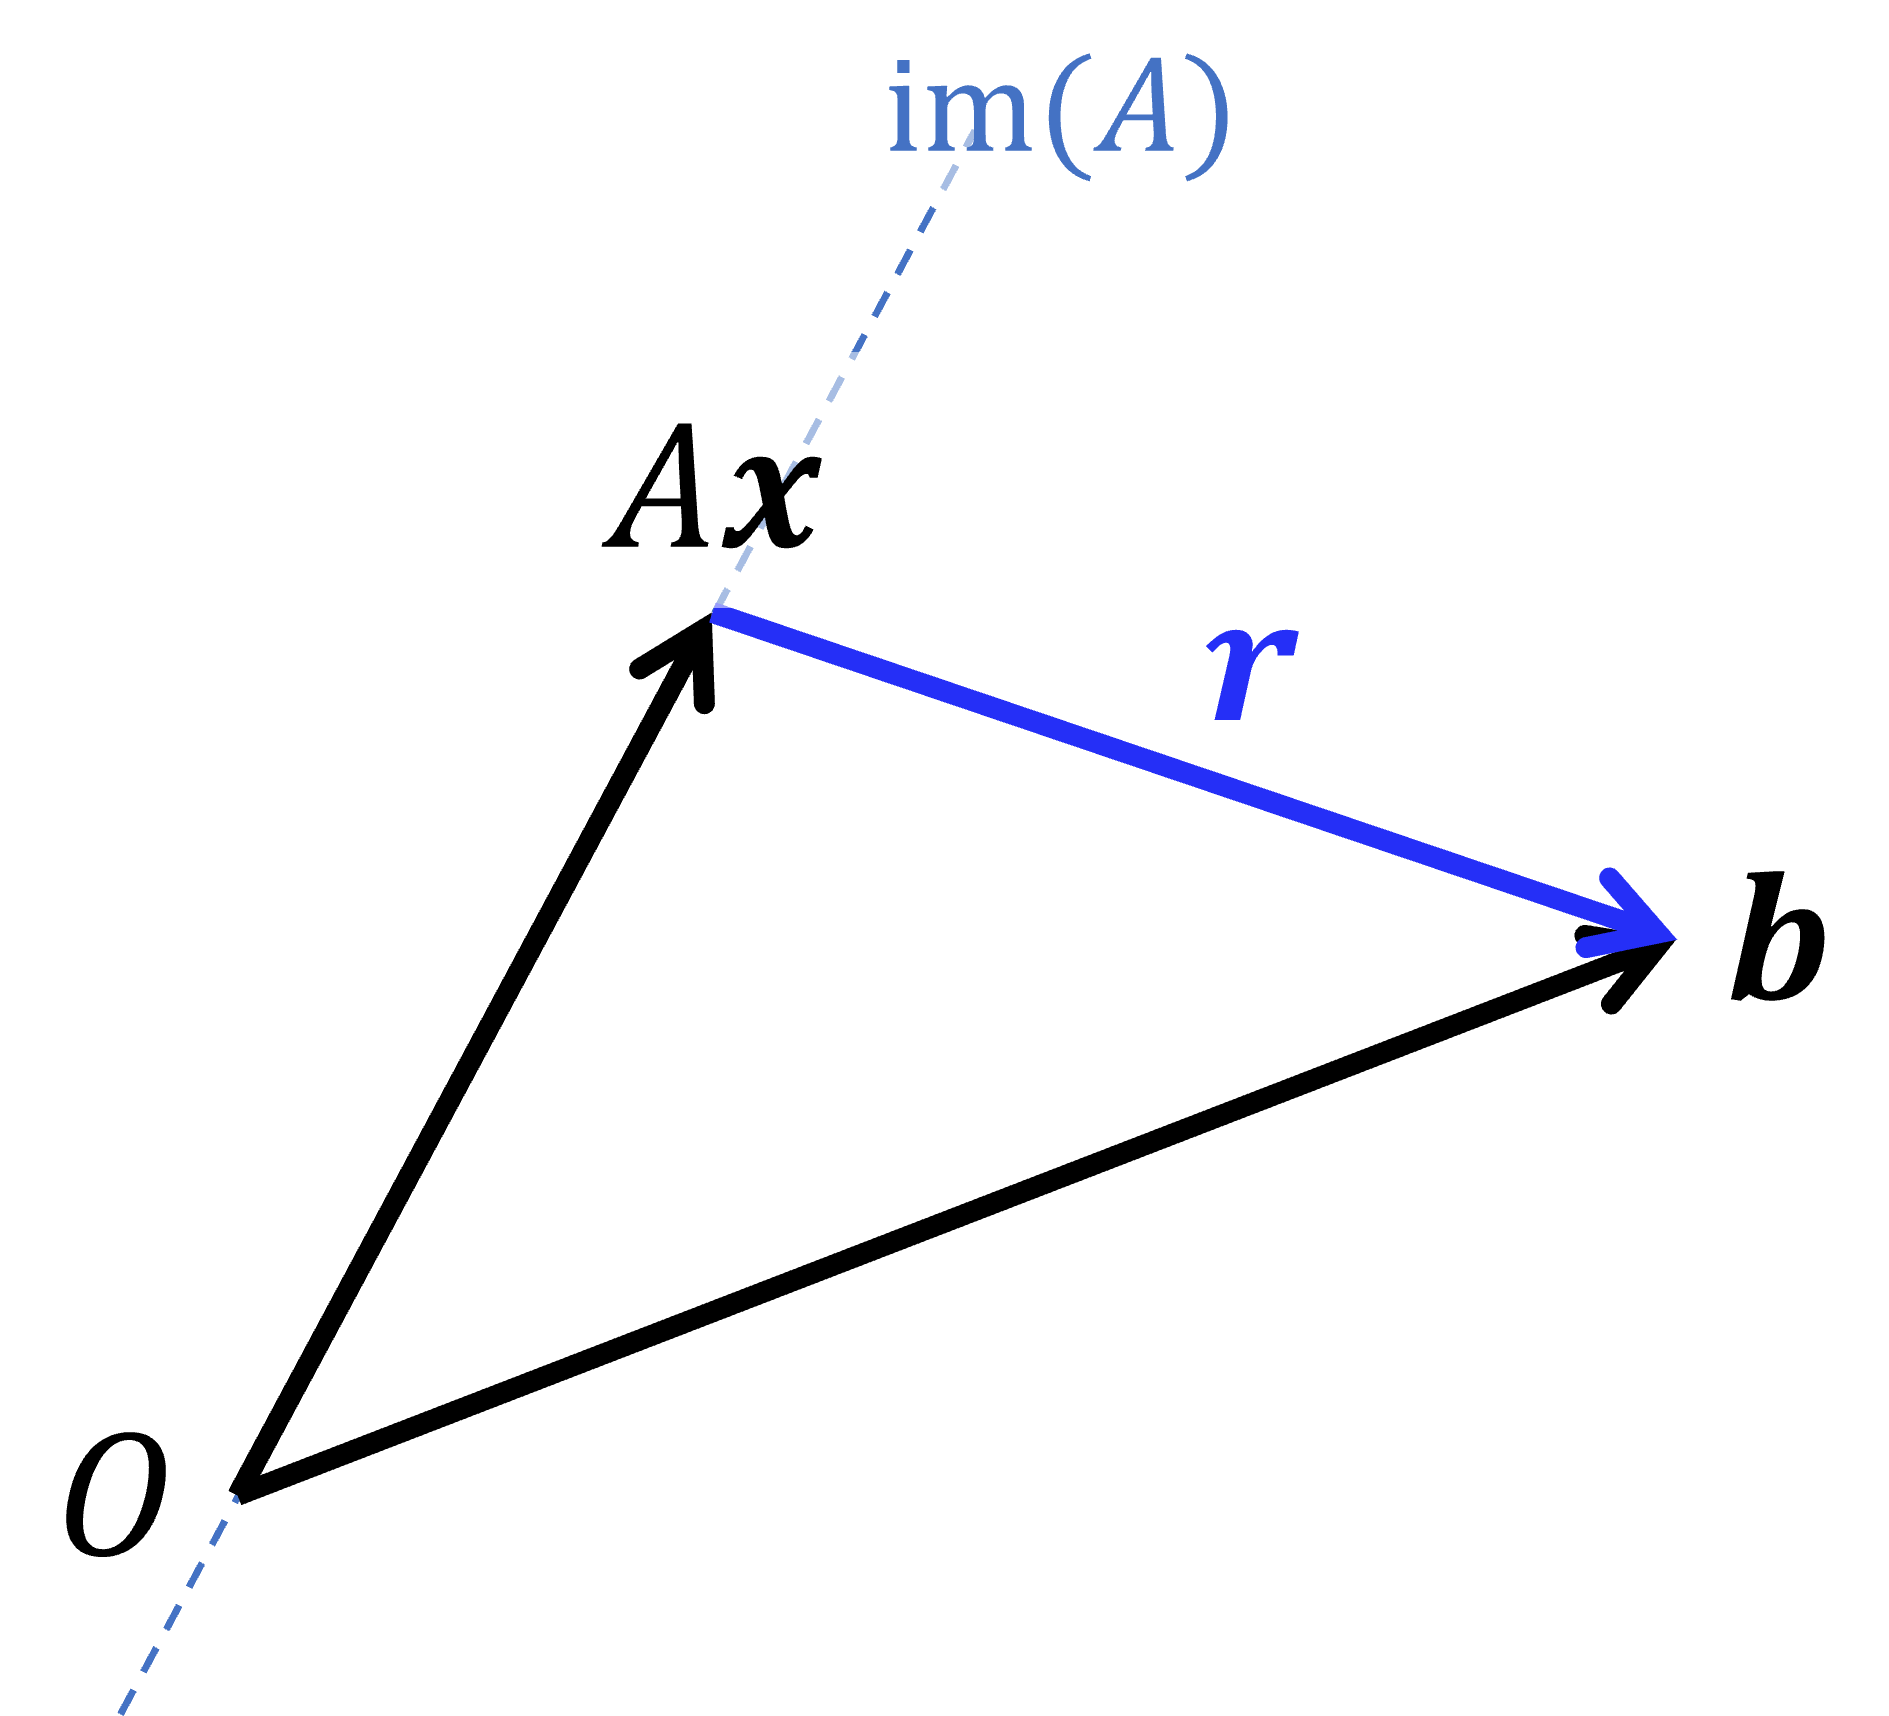
\includegraphics[width=\textwidth]{../Mathematik_2/Bilder_unused/ausgleichsrechnung_residuum_im_bildraum.png}
\end{minipage}
\begin{minipage}{0.7\textwidth}
	\begin{itemize}
		\item Ist $\vec b$ nicht im Bildraum von $A$,
existiert keine exakte L�sung.
\item Gesucht ist daher die beste Approximation im Sinne des minimalen Abstands.
	\end{itemize}
\end{minipage}
\end{exabox}
\bigskip

Wir formulieren das Minimierungsproblem:

\[
\min_{\vec x}
\|A\vec x - \vec b\|.
\]

Definiert man das Residuum

\[
	\vec r := A\vec x - \vec b\,,
\]

so gilt im Optimalfall:

\[
	\vec r \perp \mathrm{im}(A)\,.
\]

Das Element in \(\mathrm{im}(A)\), das die Orthogonalit�tsbedingung erf�llt ist die L�sung der sogenannten Normalengleichung:

\[
	A^T (A\vec x_* - \vec b) = 0\,.
\]

Die Normalengleichung ist die algebraische Formulierung der Orthogonalprojektion. Die L�sung der Normalengleichung liefert genau denjenigen Punkt im Bildraum von $A$, dessen Abstand zu $\vec b$ minimal ist. Und dass das so ist, k�nnen wir beweisen, in dem wir zeigen, dass \(\vec r \) tats�chlich orthogonal zu allen Vektoren im Bild von \(A\) ist:

\[\begin{array}{rcl l}
		\forall \, \vec x \in \mathbb R^n:\quad \langle  A\,\vec x, \vec r\rangle &=& \langle  A\,\vec x,  A\,\vec x_* - \vec b\rangle  & \| \; \textnormal{ beliebiges Element in } \mathrm{im}(A): \; A\,\vec x \\
		&=& \langle  \vec x, A^\intercal \left( A\vec x_* - \vec b \right) \rangle &\|\; \textnormal{Eigenschaft der Matrix-Vektor-Multiplikation} \\
		&=& \langle  \vec x,  A^\intercal A\vec x_* - A^\intercal \, \vec b   \rangle & \|\; \vec x_* \textnormal{ l�st die Normalengleichung: } \;   A^\intercal A\, \vec x_* - A^\intercal \, \vec b = \vec 0 \\ &=& \langle  \vec x, \vec 0  \rangle & \\ &=&  0 &
\end{array}\]


